\documentclass[11pt]{article}
\usepackage[utf8]{inputenc}
\usepackage[ngerman]{babel}

\usepackage{amsmath,amsthm,amssymb,amsfonts}

\usepackage{graphicx}
\usepackage{float}
\usepackage{tikz}

\usepackage{fancyhdr} % For headers and footers
\usepackage{geometry}
\usepackage{listings}
\usepackage{hyperref}
\hypersetup{
    linkcolor=blue,     
    urlcolor=cyan,
}

\geometry{
    a4paper, % Change this if you intend to print on a different paper size, such as letter paper.
    left=20mm,
    right=20mm,
    top=30mm,
    bottom=30mm,
}

\newcount\colveccount
\newcommand*\colvec[1]{
        \global\colveccount#1
        \begin{pmatrix}
        \colvecnext
}
\def\colvecnext#1{
        #1
        \global\advance\colveccount-1
        \ifnum\colveccount>0
                \\
                \expandafter\colvecnext
        \else
                \end{pmatrix}
        \fi
}

\title{Kinematik - Kombinierte Translations- und Rotationsbewegungen}
\author{Emil Staikov}
\date{14. Juni 2021}

\begin{document}
\maketitle
\section{Allgemeine zusammengesetzte Bewegungen}
Bis jetzt haben wir nur Bewegungen betrachtet, die reine Translationen oder Rotationen darstellen. Das ist zwar physikalisch schon interessant, die meisten echten Bewegungen sind aber zumindest auf den ersten Blick komplexer. Es stellt sich jedoch heraus, dass in starren Körpern ein besonderer Punkt existiert, der uns erlaubt, komplexe Bewegungen zu zerlegen. Dies ist der sogenannte Schwerpunkt, bei einigen Körpern ist er leicht zu ermitteln. Bei Kreisen ist er gleich dem Mittelpunkt, bei Dreiecken ist er der Schnittpunkt der Seitenhalbierenden. Sogar bei komplexen Bewegungen durchläuft der Schwerpunkt eines Körpers immernoch eine Translationsbewegung, die Bewegung der restlichen Punkte setzt sich aus der Translation des Schwerpunkts und einer oder mehrerer Rotationen um feste Achsen, die durch den Schwerpunkt gehen, zusammen. 
\begin{figure}[H]
        \centering
        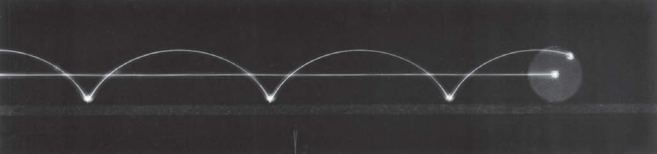
\includegraphics[width=\textwidth]{abb/5-komb-rot-tra-rollen-ohne-rutschen/schwerpunkt-translation.png}
        \caption{Ein rollendes Rad mit Lichtern am Schwerpunkt und am Rand, Abbildung aus HRK Vol. 1.}
\end{figure}
Im Bild wird erkennbar, dass sich der Schwerpunkt geradlinig bewegt, während der Außenpunkt eine komplexere Kurve durchläuft. Die Bahn, die der Außenpunkt durchläuft, wird als Zykloide bezeichnet. \\
Obowhl diese Zerlegung für viele komplexe Bewegungen möglich ist, bleibt es schwierig, die Parameter der einzelnen Teilbewegungen (also z. B. Geschwindigkeit, Beschleunigung, ... des Schwerpunkts, Winkelgeschwindigkeit, -beschleunigung, ... der verschiedenen Rotationen um den Schwerpunkt) zu bestimmen. Zusätzlich ist die exakte Bestimmung des Schwerpunkts für kompliziertere Körper teils aufwendig/nicht möglich. Bei einigen Bewegungen ergeben sich durch diese Zerlegungen jedoch interessante Zusammenhänge, eine dieser Bewegungen ist das Rollen ohne Rutschen. 


\section{Rollen ohne Rutschen}
Beim Rollen ohne Rutschen rollt ein Körper so, dass sich sein momentaner Auflagepunkt relativ zur Auflagefläche nicht bewegt. 
\subsection{Voraussetzungen}
Das sich der Auflagepunkt relativ zur Oberfläche nicht bewegt, heißt, dass er im Bezugssystem der Oberfläche Geschwindigkeit null hat. Der Berührpunkt muss auch Beschleunigung null haben, die Kräftsumme dort ist also ebenfalls null. Betrachten wir den Fall, dass ein Zylinder ohne zu rutschen eine schiefe Ebene herunterrollt. 
\begin{figure}[H]
        \centering
        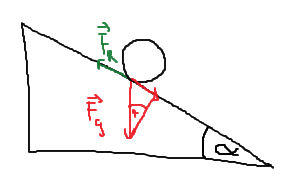
\includegraphics{abb/5-komb-rot-tra-rollen-ohne-rutschen/schiefe-ebene.png}
        \caption{Zylinder rollt ohne zu Rutschen auf einer schiefen Ebene.}
\end{figure}
Wenn wir annehmen, dass die Anfangsgeschwindigkeit des Auflagepunkts bezüglich der Oberfläche 0 ist, müssen sich die am Auflagepunkt wirkenden Kräfte ausgleichen, damit ein Rollen ohne Rutschen zustandekommt. Es muss also $F_R = \mu_RN = F_g = mg \sin\alpha$ gelten, wobei $F_R$ die Rollreibungskraft, $\mu_R$ der Rollreibungskoeffizient, $N$ die Normalkraft, $F_g$ die Gravitationskraft, $m$ die Masse des Zylinders, $g$ die Erdbeschleunigung und $\alpha$ der Öffnungswinkel der Ebene ist. Wenn wir wissen, dass es sich um ein Rollen ohne Rutschen handelt, können wir daraus umgekehrt schließen, dass $F_R = F_g\sin\alpha$. Da sich der Auflagepunkt bezüglich der Oberfläche nicht bewegt, wissen wir außerdem, dass die Reibung hier keine Arbeit verrichtet. \\ 

\pagebreak
\subsection{Kinematische Betrachtung}
Aus den Voraussetzungen für das Rollen ohne Rutschen können wir einiges über die Parameter der zusammengesetzten Bewegung schließen. Dafür finden wir zwei Ansätze. 
\subsubsection{Zerlegung in Rotation und Translation}
Wir zerlegen das Rollen ohne Rutschen in eine geradlinige Translation aller Punkte mit der Geschwindigkeit $v_S$ des Schwerpunkts, und in eine Rotation um den Schwerpunkt mit der Winkeleschwindigkeit $\omega$ bzw. Tangentialgeschwindigkeit $v_T$ ($v_T = r\omega$, wobei $r$ der Radius des rollenden Objekts ist). Diese zwei Bewegungen können wir nun addieren. 
\begin{figure}[H]
        \centering
        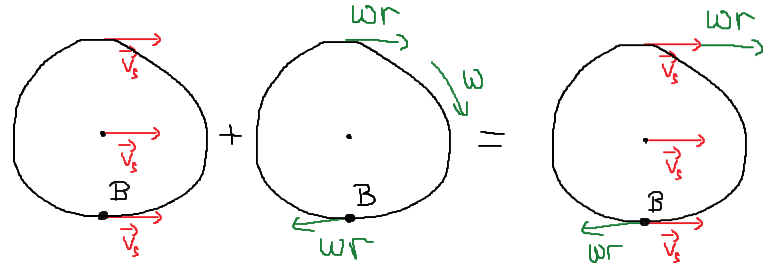
\includegraphics[width = 0.9\textwidth]{abb/5-komb-rot-tra-rollen-ohne-rutschen/kinematik-kombiniert.png}
        \caption{Zusammensetzung der Bewegung, $B$ ist der Berührpunkt.}
\end{figure}
Die Geschwindigkeit bei $B$ ist, da es sich um ein Rollen ohne Rutschen handelt, $0$. Folglich gilt 
\begin{equation*}
        r\omega + v_S = 0 \iff v_S = r\omega = v_T
\end{equation*}
In jedem gegebenen Moment ist die Geschwindigkeit des Berührpunkts dann $0$, des Schwerpunkts $v_S = r\omega = v_T$ und des äußersten Punkts $v_S + r\omega = 2r\omega = 2v_S = 2v_T$. \\
Mit dieser Überlagerungsidee können wir auch Geschwindigkeiten beliebiger Punkte des Körpers bestimmen. Diese ergeben sich zu 
\begin{align*}
        v_S + d_M\omega &= r\omega + d_M\omega = (r+d_M)\omega \\
        &= v_S + d_M\frac{v_S}{r} = \bigg(1 + \frac{d_M}{r}\bigg)v_S
\end{align*}
wobei $d_M$ der Abstand zum Schwerpunkt ist.  \\\\
Für die kinetische Energie eines Körpers, der rollt, ohne zu rutschen, gilt dann 
\begin{align*}
        E_{kin} &= E_{kin, tra} + E_{kin, rot} \\
        &= \frac{1}{2}mv_S^2 + \frac{1}{2}I\omega^2 = \frac{1}{2}m(r\omega)^2 + \frac{1}{2}I\omega^2 = \frac{1}{2}\omega^2 (I + mr^2)\\  
        &= \frac{1}{2}mv_S^2 + \frac{1}{2}I\bigg(\frac{v_S}{r}\bigg)^2 = \frac{1}{2}v_S^2\bigg(m + \frac{I}{r^2}\bigg)
\end{align*}
Das Trägheitsmoment $I$ ist hier nicht mehr gleich $mr^2$, da die Kugel kein einzelner Massepunkt ist. $I$ bezieht sich auf das Trägheitsmoment um den Schwerpunkt. 
\subsubsection{Momentane Rotationsachse}
Das Rollen ohne Rutschen können wir auch auf andere Art untersuchen. In jedem bestimmten Moment können wir die Bewegung auch durch eine reine Rotation um eine Achse durch den Berührungspunkt beschreiben. 
\begin{figure}[H]
        \centering
        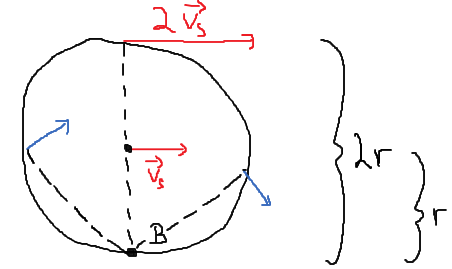
\includegraphics{abb/5-komb-rot-tra-rollen-ohne-rutschen/momentane-rot-achse.png}
        \caption{Rollen ohne Rutschen als Rotation um eine momentane Rotationsachse.}
\end{figure}
Der Schwerpunkt hat den Abstand $r$ von unserer Rotationsachse durch $B$ und bewegt sich mit der Geschwindigkeit $v_S$. Daraus können wir die Winkelgeschwindigkeit $\omega_B$ um die Achse errechnen, es gilt $\displaystyle\omega_B = \frac{v_S}{r}$. Die Tangentialgeschwindigkeit am äußersten Punkt ist dann $2r\omega_B = 2v_S$, wie durch die Überlagerung bestimmt. \\
Mit dieser neuen Perspektive auf die Bewegung können wir aber noch mehr ermitteln, da wir die Winkelgeschwindigkeit um $B$ kennen. Wenn wir jetzt noch den Abstand $d_B$ von $B$ zu einem beliebigen Punkt in dem rollenden Körper ermitteln können, bestimmen wir dessen Translationsgeschwindigkeit zu $\displaystyle d_B\omega_B = \frac{d_B}{r}v_S$.
\end{document}